\subsection{Inicialización del proyecto de Backend}
El proyecto de Backend consiste en una API realizada en el framework Express.js. Este proyecto sí es creado desde cero, por lo que se deben seguir unos cuantos pasos extra. Es importante mencionar que también debe estar ya instalado Node.js, al igual que un gestor de dependencias.

Lo primero que se tiene que hacer es crear una carpeta donde va a estar guardado todo el proyecto. Para crear una carpeta, se ejecuta el siguiente comando (puede cambiar de acuerdo al Sistema Operativo que se use):
    \begin{center}
        \textbf{
            \emph{
                mkdir nombre-carpeta
                }
            }
    \end{center}
Posteriormente, se ingresa a la carpeta y desde ahí se ejecuta el siguiente comando:
    \begin{center}
        \textbf{
            \emph{
                npm init -y
                }
            }
    \end{center}
Lo que hace ese comando es iniciar la configuración del proyecto, al usuario se le hacen ciertas preguntas para saber que cosas quiere incluir o usar. La opción -y hace que a todas las preguntas se les responda con un ``sí'', por lo que se puede omitir si se desea pensar un poco más en la configuración.

Como esta es una API realizada con Express.js, es necesario instalar el paquete. Para instalar Express.js, se ejecuta el siguiente comando:
    \begin{center}
        \textbf{
            \emph{
                npm install express
                }
            }
    \end{center}
Ahora sólo falta crear el servidor de Express, ya que ahí es donde se realizarán las diferentes solicitudes HTTP desde el Frontend. Para lograr esto, se crea un archivo que preferentemente se llame ``index.js'', aunque puede llevar cualquier nombre; en este archivo es donde se inicializa el servidor y se colocan las rutas y middlewares que vayan a ser ocupados. Para inicializar el servidor de Express, se añaden las siguientes líneas de código (Ver figura 1):

    \begin{figure}[H]
        \begin{center}
            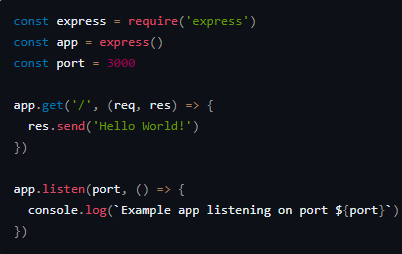
\includegraphics[scale=0.84]{img/actividades/inicializacion-despliegue/express-basic-app.png}
            \caption{Aplicación básica de Express.}
            \label{fig:express-basic-app}
        \end{center}
    \end{figure}
Y para ejecutar la aplicación, se utiliza el siguiente comando:
    \begin{center}
        \textbf{
            \emph{
                node index.js
                }
            }
    \end{center}
Con ese comando se ejecuta el servidor de manera local y se pueden realizar algunas solicitudes HTTP a la URL \emph{http://localhost:3000}.